\documentclass[runningheads]{comsis2}

\usepackage{amssymb}
\usepackage{amsmath}
\setcounter{tocdepth}{3}

\usepackage{graphicx}
\graphicspath{{./pdf/}}
\DeclareGraphicsExtensions{.pdf}

\usepackage[caption=false,font=footnotesize,labelfont=sf,textfont=sf]{subfig}
\usepackage[ruled,vlined,linesnumbered]{algorithm2e}

\usepackage{url}
\usepackage{multirow,booktabs,makecell,color,colortbl}

%% Necessary definitions for the running heads
\def\journalissue{Computer Science and Information Systems ?(?):??--??}
\def\paperidnum{DOI: N/A}
\setcounter{page}{1}

\title{A Heuristically Optimized Partitioning Strategy on Elias-Fano Index}

%% Use this if the title is too long for the running heads
\titlerunning{A Heuristically Optimized Partitioning Strategy on Elias-Fano Index}

\author{Xingshen Song \and Yuexiang Yang}


%% Use this the list of authors is too long for the running heads
%\authorrunning{First Author et al.}

\institute{College of Computer, National University of Defense Technology\\ Changsha, China\\
  \email{\{songxingshen, yyx\}@nudt.edu.cn}}

\begin{document}

\maketitle

\begin{abstract}
Inverted index is the preferred data structure for data managing and query processing in large information systems, its compression techniques have long been studied to mitigate the dichotomy between space occupancy and decompression time.
During compression, partitioning posting list into blocks while keeping aligned with its clustered distribution, can effectively minimize the compressed size while keeping partitions separately accessed.
Traditional partitioning strategies using fixed-sized blocks trend to be easy to implement, but their compression effectiveness is vulnerable to outliers.
Recently researchers begin to apply dynamic programming to determine optimal partitions with variable-sized blocks.
However, these partitioning strategies sacrifice too much compression time.

In this paper, we first compare performances of existing encoders in the space-time trade-off curve, then we present a faster algorithm to heuristically compute optimal partitions for the state-of-the-art Partitioned Elias-Fano index, taking account of compression time while maintaining the same approximation guarantees.
Experimental results on two document collections show that our method is significantly faster than its original version, at the price of a slightly worse compression ratio and query efficiency.

\vspace{6pt}\textbf{Keywords:} Inverted Index, Index Compression, Partitioning Strategy, Approximation Algorithm.
\end{abstract}

\section{Introduction}\label{sec:intro}

The performance of Information Retrieval systems relies largely on the data structure they adopt.
A well-designed data structure can juggle the mission of effectively storing related information and efficiently answering different kinds of queries.
Due to its simplicity and flexibility, inverted index gains more popularity than other candidates among modern IR systems since the 1950s \cite{buttcher2010information,witten1999managing}, especially in large scale search engines.
However, as the rapid growth of the web, inverted index is facing a formidable performance challenge by billions of increasing documents and highly-concurrent queries.
Index compression is an important technique to mitigate such problem cause it can yield a twofold advantage:
the immediate effect is that reduced space occupancy allows more data to be stored in limited store unit;
more importantly, compression makes it possible to build in-memory index thus reducing the time of data transfer from slow memories \cite{manning2008introduction,zobel2006inverted}.

Inverted index can be seen as a collection of posting lists where each list $I_t$ is mapped to one term \textit{t} of vocabulary.
Inside $I_t$ are postings containing information about the occurrences of \textit{t} in one particular document \textit{d}, typically the \textit{docid}, the \textit{frequency}, and possibly the \textit{position} and other information.
These postings are always ordered by docid or frequency to fit different IR tasks \cite{navarro2010dual}.
To facilitate both compression and query processing, each list is treated as separate data stream and components inside are stored as integers in a non-interleaved way \cite{anh2010index}.

Many techniques for inverted index compression have been studied over years, see \cite{catena2014inverted,trotman2014compression} for more details.
Among these techniques, splitting posting list into \textit{blocks} (or \textit{chunks}) has been demonstrated to be an efficient way and widely adopted by many encoders.
By keeping blocks separately accessible we can expect faster decoding speed and hierarchical structure.
In addition, variable-sized blocks can utilize the clustering property of list to beat the entropy \cite{silvestri2010vsencoding,moffat2000binary}.
However, finding optimal partitions using variable-sized blocks can be very time consuming and the decoding procedure is delayed by additional cache miss.

While state-of-the-art techniques do obtain excellent space-time trade-offs, compression time is always neglected as one evaluating criterion.
This can be attributed to the fact that index is always preprocessed offline before deployment, and once being taken into effect, update can be committed in an asynchronous and parallel manner.
However, timely update is becoming more and more stringent in search engine, encoders which spend much time building index may not fit this scenario anymore.
Until recently researchers begin to use breakthroughs in compact data structure to bear on problems of optimizing inverted index \cite{navarro2010dual,petri2014score}.
The newly proposed Partitioned Elias-Fano index (PEF), introduces a new representation of inverted index storing the complete form rather than differences (or \textit{gaps}) between adjacent values \cite{ottaviano2014partitioned,vigna2013quasi}.
It is shown that this kind of index supports fast random access and search operation.
An optimal partitioning strategy is also adopted using approximation algorithm, theoretically guaranteeing a solution at most $\left(1+\varepsilon\right)$ times larger than the best one can be found in linear-time, for any $ \varepsilon \in \left(0, 1\right) $.

In this paper, we show that many encoders are far from optimal in terms of compression time.
While PEF yields a better trade-off than others, its compression procedure is still too slow compared with existing partitioning strategies using fixed-sized blocks, for the reason that the index size and the query efficiency of PEF heavily depends on the carefully tuned parameters.
Even after the parameters configured, the time needed to build an inverted index on GOV2 using multi-thread is nearly one hour while other encoders may only cost around ten minutes.
There is still much potential for the compression speed of PEF to be improved.
We provide a heuristic partitioning strategy on PEF which computes partitions in a single pass with only one sliding window.
More precisely, we compare the sizes of a series of adjacent blocks, once an exceptional small block is detected, an endpoint then will be assigned inside it, based on an observation that block length should grow in proportion as its space cost.
Last we perform an experiment on two collection, GOV2 and Common Crawl, which shows the compression time is significantly reduced against the original work while its space occupancy and decompression time maintains comparable to the original one.
\section{Index Compression and Partitioning Strategies}\label{sec:background}

Compressing the index has long been a key issue for researchers to ensure both the time- and space-efficiency of inverted index, various encoders with different properties have been put up to settle this problem, and they can be roughly divided into two classes, namely the \textit{integer-oriented encoders} and the \textit{list-oriented encoders}.

The integer-oriented encoders assign a unique codeword to each integer of the input list, then the compression procedure turns into a mapping or substitution from the integer space to code space.
As they compress integers without considering their neighbors, the integer-oriented encoders are also called oblivious encoders \cite{catena2014inverted}, such as \textit{unary code, Elias Gamma/Delta codes \emph{and} Golomb/Rice codes}.
Most integer-oriented encoders are hard to decode since they need bitwise operations to cross computer word boundaries, so byte/word-aligned encoders, are proposed to solve this problem, like \textit{Variable Byte} and \textit{Group Varint}, more importantly, they can be further improved by SIMD instructions of modern CPUs \cite{stepanov2011simd,trotman2014compression}.

List-oriented encoders are designed to exploit the cluster of neighboring integers, each time a fixed-sized or variable-sized group of integers is binary packed with a uniform bit width, providing equivalent compression ratio and faster decoding speed, the technique used by these encoders is called \textit{frame-of-reference}(FOR), or \textit{binary packing} \cite{goldstein1998compressing}.
Basically, their compression ratios are inferior to these of the first category due to the fact that a batch of integers are encoded indiscriminately, and useless zeros are filled in the codeword to keep word-aligned.
However, when decoded, list-oriented encoders can obtain an entire block while the formers just decode one integer at a time.
More importantly, with the help of \textit{skip pointers} or \textit{skip list}, it is possible to step along the codewords compressed by list-oriented encoders and stop when the required number of blocks has been bypassed.
Some of these encoders are \textit{Simple Family}, AFOR and \textit{Patched} FOR (PFOR, OptPFOR and FastPFOR).

%\paragraph{Directed Acyclic Graph}
\textit{Directed Acyclic Graph.}
One thing to be noted is that list-oriented encoders may cost equivalent time to compress the posting list as the integer-oriented encoders even they are designed to compress a list of integers at the same time.
Before compressing, a partitioning strategy is needed to traverse the whole input list to search for an optimal partition, in consideration of compression ratio and decoding speed.
Even after that, a uniform bit width has to be chosen to fit every element in for each block.
Compression techniques like the Simple Family \cite{anh2005inverted,anh2010index}, enumerates all the possible partitioning cases to choose the suitable decision; OptPFOR \cite{yan2009inverted} needs an additional computation to choose the optimal proportion of exceptions in each block in order to achieve a better space efficiency.
In the last few years there is a surge of partitioning schemes to accelerate the compression procedure \cite{lemire2015decoding,ottaviano2014partitioned,zhao2015general}.

There is a common view that traditional methods which use a fixed-sized block to uniformly partition a sequence fail to exploit the nature of the underlying sequence, that the list is formed by clusters of consecutive integers.
Indeed, the sequence contains postings of documents crawled from different domains, when the docids are reordered by their URLs, more and larger clusters of integers which are very close to each other will show up.
We cannot expect uniform partitioning to be optimal since clusters are not likely to be aligned with each fixed-sized block.
A more practical way to enhance compression efficiency is to use blocks with variable size to adapt the encoding to the integer distribution.

AFOR and method proposed by \cite{anh2004index} give an initiative trial on optimal partitioning scheme.
AFOR breaks a fixed-sized block into multiple frames of variable length, and arrange different combinations to achieve better compression.
It does get an impressive compression speed in our experiment, however, its partitioning scheme is quite rough as few options for frame length provide a limited performance.
% and finds a reasonable trade-off by defining the block size to 32 with three frame lengths, 32, 16 and 8, each time a block is fetched and combinations of the three frames are evaluated to encode this block.
\cite{anh2004index} uses a similar technique as AFOR, but encodes the sequence under static table driven approaches, namely deciding the optimal partition by looking up a predefined table and comparing different options.
The option chosen for the current partition is always adjacent to the last-used one in the table, thus minimizing the space occupied by descriptor.
However, this encoder outputs bit-aligned codes which are inefficient to write and read.
VSEncoding further extends AFOR with more flexibility to partition a sequence via bottom-up dynamic programming approach, which also brings a side effect that the time and space complexity turns into polynomial, making this solution prohibitive.
Several variant implementations are provided on its website\footnote{\url{http://integerencoding.isti.cnr.it/}}, for example, VSE-R achieves the best compression ratio and VSE-Simple achieves the best decoding speed.
The recently proposed PEF sheds light upon how to accelerate the compression performance of VSEncoding with approximation algorithms, PEF identifies the minimum-space partition by omitting inefficient schemes, thus time complexity is greatly reduced.
\begin{figure}
	\centering
	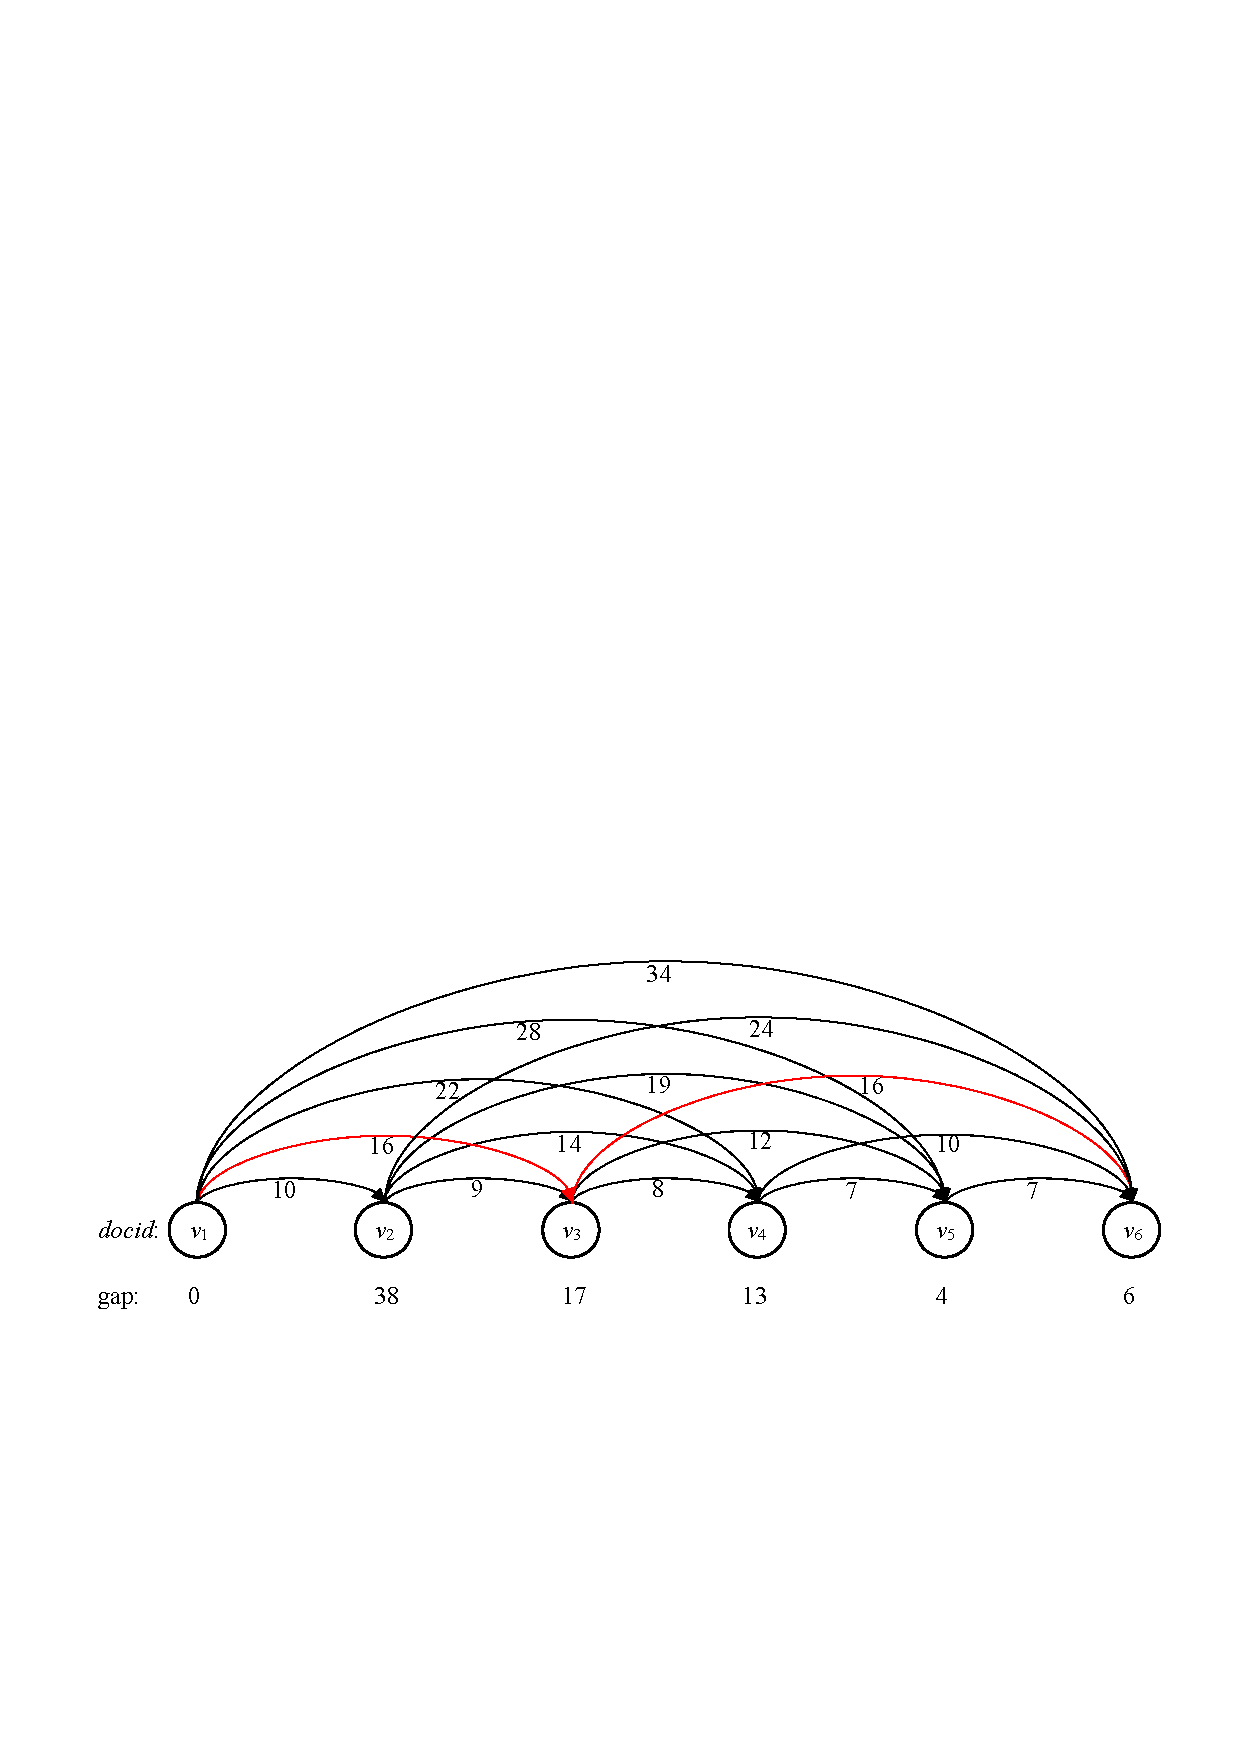
\includegraphics[width=0.9\linewidth]{sssp}
	\caption[sssp]{Here is a DAG for sequence with 6 docids, with each vertex represents a docid, and each edge represents a block containing docids along the edge. The docids, denoted as vertexes, are represented using gaps. The number under the edge denotes the cost for it, which is calculated by summing fixed cost of building a block (here it is set to be 4) and bits to encode the block. Red lines are the shortest path for this graph, namely, the optimal partition with the smallest space cost.}
	\label{fig:sssp}
\end{figure}

The common foundation for the abovementioned methods is to recast the integer sequence $\mathcal{S} \left[ 0, n \right]$ to a particular DAG $\mathcal{G}$, each integer is represented by a vertex $ v $, plus a dummy vertex marking the end of the sequence.
The graph $\mathcal{G}$ is complete, which means that for any $i$ and $j$ with $i < j \leqslant n$, there exists an edge connecting $v_{i}$ and $v_{j}$, denoted as $\left( v_{i}, v_{j} \right)$.
In fact, the edge is an exact correspondence of a partition in the sequence $\mathcal{S}\left[i, j \right] $, the problem of fully partitioning $\mathcal{S}$ is converted to finding a path $\pi$ in $\mathcal{G}$, for instance, $\pi=\left( v_{0}, v_{i_{1}} \right) \left( v_{i_{1}}, v_{i_{2}} \right)\ldots\left( v_{i_{k-1}}, v_{n} \right)$ with $k$ edges corresponds to the partition $\mathcal{S}\left[0, i_{1}-1 \right]\mathcal{S}\left[i_{1}, i_{2}-1 \right] \ldots\mathcal{S}\left[i_{k-1}, n-1\right] $ of $k$ blocks.
The weight of an edge in the graph is equal to the cost in bits consumed by the partition.
Thus, the problem of optimally partitioning a sequence is reduced to the problem of Single-Source Shortest Path(SSSP) Labeling, as shown in Fig.~\ref{fig:sssp}.
An intuitive way to solve this is to firstly set the cost of each vertex in $\mathcal{G}$ to $+\infty$, then an iteration starts from the left vertex to the rightmost, when it comes to a vertex $v_{j}$ with $0\leqslant j < n$, a subproblem of find the optimal path from $v_{j}$ to $v_{n}$ shows up, assuming the optimal path from $v_{0}$ to $v_{j}$ has been correctly computed.
Each edge $\left( v_{j}, v' \right)$ outgoing from $v_{j}$ will be assessed and cost of vertex $v'$ is updated if it becomes smaller.
As can be seen, the time complexity of this algorithm is proportional to the number of edges in $\mathcal{G}$.

However, the $\mathcal{G}$ transformed from integer sequence $\mathcal{S}$ is complete with $\Theta\left( n^{2}\right)$ edges, especially some posting lists for popular terms will be quite large, finding their optimal partitions will be intolerable.
Since dynamic programming is inefficient and greedy mechanism is too coarse, a more feasible way will be using an elaborate approximation algorithm to find slightly suboptimal solutions, which reduce the time and space complexities to linear.
%SXS: Reduced Version of the Above paragraphs
%Blocks with fixed length are likely to be suboptimal as integers in posting list will not be evenly distributed.
%Works from literature \cite{anh2004index,delbru2012searching,silvestri2010vsencoding} give another perspective on partitioning.
%The posting list $\mathcal{S}[0, n-1]$ is considered a particular directed acyclic graph $\mathcal{G}$, each integer is represented by a vertex $v$, edge denoted as $\left( v_{i}, v_{j} \right)$ is an exact correspondence of a partition in the posting list $\mathcal{S}\left[i, j \right]$, edge has also associated its cost $c(v_{i}, v_{j})=\left| \mathcal{E}\left(\mathcal{S}\left[i, j-1 \right] \right) \right| $ that corresponds to the size in bits of the partition compressed by encoder $\mathcal{E}$.
%Thus, the problem of optimally partitioning a list is reduced to the problem of Single-Source Shortest Path(SSSP) Problem.
%		
%However, a trivial traversal may not suffice to obtain an efficient solution for this problem, as the graph $\mathcal{G}$ is complete with $\Theta\left( n^{2}\right)$ edges, even partitioning posting lists with thousands of integers will be intolerable.
%Anh et al. \cite{anh2004index} and Delbru et al. \cite{delbru2012searching} adopt a greedy mechanism to partition the lists, the difference between them is that the former partitions the lists under a static table driven approach while the latter uses a set of fixed-sized sliding windows to determine.
%Fabrizio \cite{silvestri2010vsencoding} finds the optimal partition under a \textit{dynamic programming} approach but with limited options for partition lengths (say \textit{h}), reducing its time complexity from $O(n^{2})$ to $O(nh)$, but still barely satisfying in practice.
%		
%Since dynamic programming is inefficient and greedy mechanism is too coarse, a more feasible way will be using an elaborate approximation algorithm to find slightly suboptimal solutions, which reduce the time and space complexities to linear.

\section{Method Evaluation Criteria}\label{sec:criteria}

Compression techniques are optimized under two criteria, namely \textit{decompression time} and \textit{space occupancy}.
Different encoders yield different space-time trade-offs, generally, integer-oriented encoders tend to be more space-efficient while list-oriented encoders focus on time efficiency.
\textit{Compression time} stays a low profile in the literature, as it does not make a difference for practical use, many encoders pursue a better performance at the expense of prolonging compression time.
Recently it begins to gain attention as one criterion to evaluate a compression technique \cite{lemire2015decoding,ottaviano2015optimal}.

\textit{Pareto-Optimal Compression.}
Taking the compression time into account, we get an extended tri-criteria to evaluate the performance of compression techniques.
In this respect, we recall the concept of \textit{Pareto-optimal} compression to define the notion of ``best" compression in a principled way, i.e., encoders achieve different points in the space-time trade-off curve.
Optimal ones are those extreme points whose performances are not worse than others in one dimension, and if to be optimized in any dimension, performances in the other two will get impaired accordingly.
Absolutely there exists a set of Pareto-optimal compressions with different considerations.
Figure~\ref{fig:performance} shows performances of different compression techniques\footnote{The installation of these implementations is same with the Experiments Section, even quite different from results in other work, but they are directly comparable with each other.}.

\begin{figure}
	\centering
	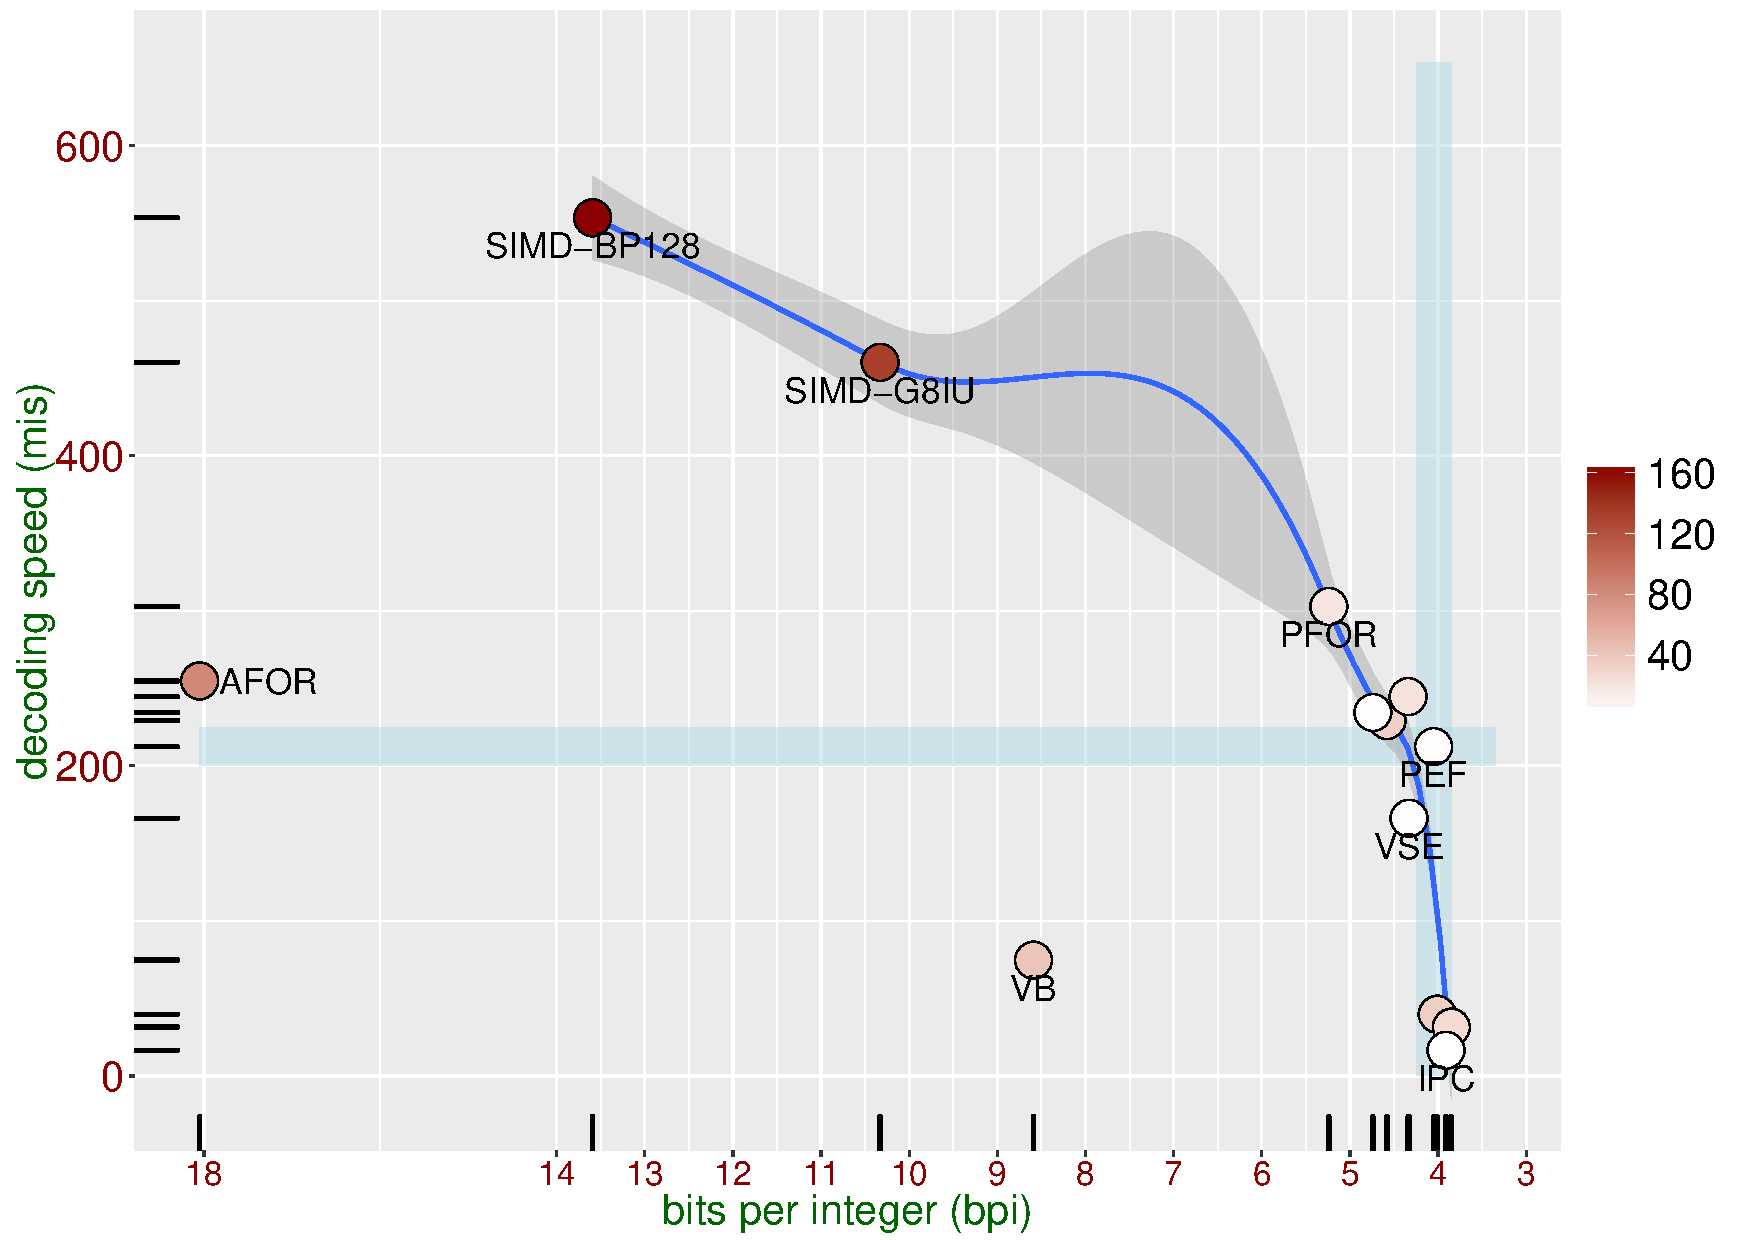
\includegraphics[width=0.7\linewidth]{performance}
	\caption{Performance of different encoders under tri-criteria. The x-axis (bpi) is arranged in a reverse order and color of each point indicates the encoding speed, the deeper, the faster.}
	\label{fig:performance}
\end{figure}

From the fitting curve and the marginal rugs, we can observe that points, which approach to limit of one dimension, begin to cluster and performances of the other two dimension drop intensely.
Points beyond the curve are either superior or inferior to the average (i.e., VB and AFOR).
Generally, these points cluster into three slots according to their decoding speed, broadly consistent with three stages in the evolution of index compression technologies.
The first stage is integer-oriented encoders proposed in early years, whose purpose is to create the smallest index, regardless of the decoding speed.
Points represent these encoders can be found at the bottom right conner.
Note there is one exception that IPC is a list-oriented encoder proposed by Moffat \& Stuiver \cite{moffat2000binary}, however, it reaches the best compression at the cost of worst decoding speed.
The second stage falls into the slot above the first one, encoders begin to pursue faster decoding speed with slightly worse compression ratio.
We can observe that these encoders even get slower compression speed than those of the first stage.
The classical Variable Byte and AFOR both get favorable encoding and decoding speed, however, with prohibitive space occupancy, especially the latter one.
%XXX: say something about the three generations of encoders, refering to paper "compression, simd and posting list"
The third stage are encoders reinforced by SIMD instructions, obtaining faster speed in encoding and decoding, but further more space.
This kind of encoders tend to occupy more spaces because it is designed to process data in bulk, namely fitting more integers into one block.
Using SIMD is superior in encoding/decoding as a whole, however, when accessing a specified position or element, more data have to be decoded.

%\textit{Partitioned Elias-Fano Index.}
We also emphasize PEF by two straight lines in Figure~\ref{fig:performance}, as it reaches a space occupancy competitive with integer-oriented encoders while keeping a reasonable decoding speed.
More importantly, it is reported to be efficient in random access and search operations but slow in sequential decoding \cite{ottaviano2015optimal,vigna2013quasi}.

PEF describes a suboptimal partitioning strategy which finds the solution in linear time by generating a pruned DAG on the posting list.
However, it is still prohibitive in compression time, because the compressed size and decoding performance of the index rely heavily on the approximation factors, to obtain the best solution these factors need to be carefully engineered for different collection.
Next section we describe a faster algorithm preserving the same approximation guarantee.

\section{Linear Partitioning Strategy}\label{sec:our method}
%XXX should I supplement pseudo code of PEF?
\subsection{Partitioned Elias-Fano Index}

Partitioned Elias-Fano Index is a two-level data structure which partitions the posting list into Elias-Fano (EF) represented \textit{chunks} to adapt to its local statistics and stores pointers to these chunks in the upper EF sequence.
The EF representation is an efficient quasi-succinct representation for monotone sequences used in \cite{elias1974efficient,vigna2013quasi}.
Given a monotonically increasing sequence $ \mathcal{S}[0, n-1] $ of $ n $ integers drawn from the range $ [0, u] $, and $ u $ is called an \textit{universe} of $ \mathcal{S} $.
$ \mathcal{S} $ is represented using two bit arrays, namely \textit{the higher bits} and \textit{the lower bits}.
For a given integer $ \ell $, each element of $ \mathcal{S} $ is split into the lower $ \ell $ bits and the higher $ \lceil \log u \rceil - \ell$ bits.
The lower bits are stored explicitly and contiguously in the lower bits array \textit{L}, the higher bits are stored in the higher bits array \textit{H} as a sequence of unary-coded gaps (\cite{ottaviano2014partitioned} uses unary-coded buckets instead, but they both reach the same space complexity).
Thus, representing \textit{L} needs exactly $ n\ell $ bits, \textit{H} needs $ n + \frac{\lceil u \rceil}{2^{\ell}} $ bits.
It has been shown that setting $ \ell = \lfloor \log \frac{u}{n} \rfloor $ minimizes the overall space of $ \mathcal{S} $, namely, at most $ n \lceil \log \frac{u}{n} \rceil + 2 n $ bits.
Elements in Elias-Fano represented sequence are directly accessible by performing unary read on \textit{H} and direct read on \textit{L}, then merging them together.

However, Elias-Fano fails to exploit the distribution of clusters in the sequence as it treats $ \mathcal{S} $ as a whole.
We can actually expect for a better space occupancy when the sequence is formed by clusters of integers which are very close to each other.
This observation motivates the introduction of a two-level Elias-Fano, namely PEF, in which $ \mathcal{S} $ is first partitioned into chunks with variable lengths, then pointers to the head of each chunk are grouped together using Elias-Fano representation.
Partitioning the sequence aligning to its clusters will definitely narrow down the average distance of consecutive elements inside, thus a smaller compressed size is possible.
An optimal partition must satisfy the following two requirements: on the one hand, the chunks should be as large as possible to minimize the number of pointers in upper level; on the other hand, the chunks should be as small as possible to narrow down the average distance.
However, traditional dynamic programming methods like \cite{silvestri2010vsencoding} turn out to be very costly when finding the optimal solution.
A more feasible way is adopting an approximation algorithm to prune the complete graph $ \mathcal{G} $ under some criteria, retaining its shortest path while cutting out edges which are less possible to be involved in space-efficient partitions.

Recall the approximation algorithm adopted in PEF, whose core idea is to generate a pruned subgraph $\mathcal{G}_{\varepsilon}\left(\mathcal{S}\right)$ of the original $\mathcal{G}\left(\mathcal{S}\right)$.
To construct $\mathcal{G}_{\varepsilon}$ on the fly, a dynamic data structure is deployed which maintains a set of \textit{sliding windows} over $\mathcal{S}$ denoted by $\omega_{0},\omega_{1},\dots, \omega_{\log_{1+\varepsilon_2}\frac{1}{\varepsilon_1}}$, each of them represents a cost class of $F\left(1+\varepsilon_2\right)^{i}$ for each integer $i$ ($F$ is the fixed cost of one partition and $\varepsilon_{2}\in\left( 0, 1 \right)$).
By setting an upper bound $U$ (say, $U=\frac{F}{\varepsilon_{1}}$ by a predefined $\varepsilon_{1}\in\left(0, 1\right)$), the total number of edges in $\mathcal{G}_{\varepsilon}\left(\mathcal{S}\right)$, addressed as $\varepsilon$-maximal edges, are $O\left(n\log_{1+\varepsilon}\frac{1}{\varepsilon}\right)$.
Thus, it is able to identify the minimum-space partition up to a small approximation factor $ \varepsilon $ within linear time.

\subsection{Heuristically Finding Optimal Partition}

These $\varepsilon$-maximal edges can be found by keeping $k = O\left(\log_{1+\varepsilon}\frac{1}{\varepsilon}\right)$ sliding windows over $\mathcal{S}$.
During the algorithm visits posting list, the sliding windows are actually potential partitions, which start at the same position $ v_{i} $ but have different lengths.
At first, all these windows are docked at vertex 0 with 0 length.
Each time as the algorithm visits a subsequent vertex, these windows expand their sizes by appending this vertex to the end, once cost of the vertexes within current window, say $ \omega_{i} $, exceeds its threshold $ F \left( 1 + \varepsilon \right) ^{i} $, $ \omega_{i} $ stops expanding its size and we get one $\varepsilon$-maximal edge of class $ i $.
Windows $ \omega_{i+1}, \dots, \omega_{k}$ will keep repeating this procedure until all the $\varepsilon$-maximal edges out going from the starting vertex are figured out.
Then algorithm repeats the above procedure to find $\varepsilon$-maximal edges for next vertex until reaches the end.

The key to keep algorithm finishing in linear time is that, these windows never contract after expanding.
Thus, for all the starting vertex we only need to evaluate few vertexes nearby the end of each window, and the only exception is vertex 0, where each sliding window has to evaluate vertexes one by one until the cost upper bound is reached.
The whole procedure can be visualized by imagining a set of elastic ribbons with different lengths being stretched along a line.
Initially, these ribbons are relaxed with both ends nailed to the starting vertex, then one end is stretched rightwards along the line.
When a ribbon is fully stretched, we nail its tail end to the current place and relax it by advance its head end one step towards right, then again stretch its tail end and so on.
Given the fact that cost calculation can be done in constant time, it is easy to prove that returning an optimal partition only needs almost $ 2n\log_{1+\varepsilon}\frac{1}{\varepsilon} $ calls to cost calculation, namely in $O\left(n\log_{1+\varepsilon}\frac{1}{\varepsilon}\right)$ time.

However, it is still inefficient in practice since there can be tens of sliding windows, and different combinations of parameters $ \varepsilon_1,\varepsilon_2 $ have to be tested before adoption.
Actually we need only one window to accommodate as many as possible integers and stop expanding as soon as an \textit{exception} is encountered.

The following lemma states a crucial property of the path over $\mathcal{G}\left(\mathcal{S}\right)$ to base our partitioning strategy on:	given any triple of indexes $i$, $j$ and $k$ in $\mathcal{G}$ with $0\leqslant i<j<k\leqslant n$, we have $c(v_{i}, v_{j})\leqslant c(v_{i}, v_{k})$ and $c(v_{j}, v_{k})\leqslant c(v_{i}, v_{k})$.
We denote edges that start from $v_{i}$ over $\mathcal{G}_{\varepsilon}\left(\mathcal{S}\right)$ as $(v_{i}, v_{j_{0}})$, $(v_{i}, v_{j_{1}})$, \ldots, $(v_{i}, v_{j_{k}})$, and for any adjacent two edges the ratio between them is $(1+\varepsilon_{2})$.
We speculate the lengths between them should also follow some regulations, an exception can enlarge the average distance inside an edge in a sudden, if to keep its weight proportional to its former one, current edge's incremental length has to be comparatively small.
However, edges without exceptions should have their edge lengths growing proportionally.
A chunk that contains exception can be found by sequentially traversing these edges and comparing the incremental lengths.
Intuitively, an exception always leads to a short interval, and once we find this kind of interval a chunk can be built inside it, thus omitting exhaustive traversing all edges from one vertex to figure it out.
We can further shift the head of sliding window to the end of current chunk to skip more calculations.
An example of the above procedure is shown in Figure~\ref{fig:exceptions}.

\begin{figure}
	\centering
	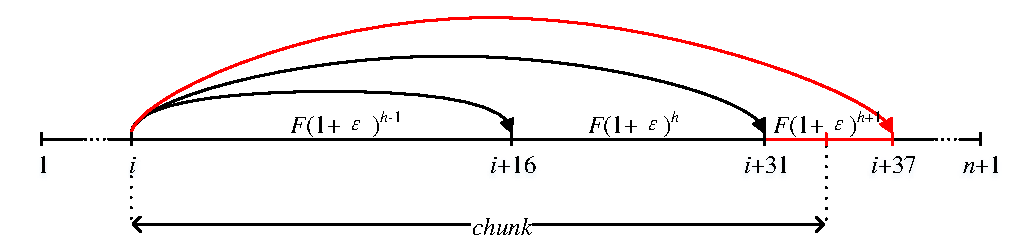
\includegraphics[width=0.9\linewidth]{exception}
	\caption{Finding $\varepsilon$-maximal edges for position $ i $ using sliding windows. Here we show three edges with cost upper bound as $ F(1+\varepsilon)^{h-1}, F(1+\varepsilon)^{h}, F(1+\varepsilon)^{h+1} $, and their edge lengths are 16, 15, 6, respectively. Then we certain that an exception is encountered inside the third edge, and we can build a chunk right before the exception to save more space and reduce calculation.}
	\label{fig:exceptions}
\end{figure}

It remains to describe how to locate the chunk which contains exceptions, given a chunk $\left(v_{i}, v_{j_{h}}\right)$, we only consider comparing with its former one, namely $\left(v_{i}, v_{j_{h-1}}\right)$, inspired by Markov process.
Thus, we have their partition lengths and partition universes as follows:
\begin{align}
n_{h} &= j_{h}-i, & u_{h} &= v_{j_{h}} - v_{i} \label{equ:chunk h}\\
n_{h-1} &= j_{h-1}-i, & u_{h-1} &= v_{j_{h-1}} - v_{i}\label{equ:chunk h-1}
\end{align}
and their bit costs
\begin{equation}\label{equ:cost ratio}
{c\left(v_{i}, v_{j_{h}}\right)}/{c\left(v_{i}, v_{j_{h-1}}\right)}=1+\varepsilon_{2}
\end{equation}
However, different encodings are used in PEF to overcome the space inefficiencies of Elias-Fano in representing dense chunks.
A chunk $ \mathcal{P}_{h} $ is called a dense chunk if it covers a large fraction of the elements in the universe, that is $ n_{h} $ is close to $ u_{h} $.
As stated before, it will cost Elias-Fano $ n_{h} \lceil \log \frac{u_{h}}{n_{h}} \rceil + 2 n_{h} $ bits to represent $ \mathcal{P}_{h} $, nearly $ 2 u_{h} $ for a dense chunk.
In this case, a bitvector with a length $ u_{h} $ bits is a better choice, $ \mathcal{P}_{h} $ is represented by setting positions where integers happen to one.
And traditional \textit{rank/select} are also easy to implemented.
Another extreme case is that chunk covers all the elements of universe $ u_{h} $, then we just need to store the partition length and partition universe while leaving the chunk non-encoded.
In spite of it is a fairly rare occurrence, once occurs it does sharply reduce the space occupancy.

To sum up, there are three representations of $ \mathcal{E} $s for different chunks.
\begin{enumerate}
	\item $ \mathcal{E}=0 $: \textit{non-encoding} with $c\left(v_{i}, v_{j_{h}}\right)=0$, if partition length $n_{h}$ equals to the universe $u_{h}$;
	\item $ \mathcal{E}=1 $: \textit{bitvector} with $c\left(v_{i}, v_{j_{h}}\right)=u_{h}$, if $n_{h}\geqslant \frac{u_{h}}{4}$;
	\item $ \mathcal{E}=2 $: EF with $c\left(v_{i}, v_{j_{h}}\right)=n_{h}\lceil\log \frac{u_{h}}{n_{h}}\rceil+2n_{h}$, if $n_{h}<\frac{u_{h}}{4}$.
\end{enumerate}
%$ \mathcal{E}=0 $: \textit{non-encoding} with $c\left(v_{i}, v_{j_{h}}\right)=0$, if partition length $n_{h}$ equals to the universe $u_{h}$; $ \mathcal{E}=1 $: \textit{bitvector} with $c\left(v_{i}, v_{j_{h}}\right)=u_{h}$, if $n_{h}\geqslant \frac{u_{h}}{4}$ and $ \mathcal{E}=2 $: EF with $c\left(v_{i}, v_{j_{h}}\right)=n_{h}\lceil\log \frac{u_{h}}{n_{h}}\rceil+2n_{h}$, if $n_{h}<\frac{u_{h}}{4}$.
When we are about to identify chunks contain exceptions, we have to enumerate all the possible combinations of two consecutive chunks to find out corresponding reasonable incremental lengths.
That is, given Eq.~\eqref{equ:chunk h}~\eqref{equ:chunk h-1}~\eqref{equ:cost ratio}, we need to calculate $ \frac{n_h}{n_{h-1}} $ for $ \mathcal{E}[h-1] $ and $ \mathcal{E}[h] $, $ \mathcal{E} \in (0, 1, 2) $.
Actually there are only 4 combinations to consider since \textit{non-encoding} is unlikely to be leaded by the other two and more sensitive to exceptions.

Take $ \mathcal{E}[h-1]=1 $ and $ \mathcal{E}[h]=2 $ for example, then
\begin{displaymath}
\noindent
1+\varepsilon_{2}=\frac{n_{h}\lceil\log \frac{u_{h}}{n_{h}}\rceil+2n_{h}}{u_{h-1}}\geqslant \frac{n_{h}}{n_{h-1}}\cdot \frac{2+\log \frac{u_{h}}{n_{h}}}{4}>\frac{n_{h}}{n_{h-1}}.
\end{displaymath}
Others get the same conclusion by deduction (See the whole procedure in APPENDIX), so we set
\begin{equation}
\frac{u_{h}}{n_{h}}=1+\varepsilon_2
\end{equation}
as the same approximation factor with that of $\varepsilon$-maximal edges.
Thus the whole procedure, which can be done within a single pass, is recast into using one window to expand its size from a starting vertex, building a chunk when current $\varepsilon$-maximal edge is $\left(1+\varepsilon_{2}\right)$ times larger than the previous one and moving the starting vertex to $v_{h-1}+1$.
A more space-efficient way is to traverse the interval $\left(v_{h}, v_{h-1}\right)$ to determine a better cut-off vertex, which increases time complexity by no more than $\left(1+\varepsilon_{2}\right)$, and a minimum partition length is set to 8 to avoid slow-start and fragmentation of chunks.
Pseudo code of the above space-efficient procedure can be found in Algorithm~\ref{alg:optimal partition}.

\begin{algorithm} \label{alg:optimal partition}
	%	\SetAlgoNoLine
	\caption{Optimal partitioning}
	\KwIn{Posting list $ \mathcal{S}\left[1, n+1\right] $, fixed cost $ F $ and approximation factor $ \varepsilon_1, \varepsilon_2 $}
	\KwOut{Vector of optimal Partition $ P $}
	Initialize sliding window $ w $, $ bounds=\left\lbrace F, F(1+\varepsilon_2), F(1+\varepsilon_2)^2,\dots, \frac{F}{\varepsilon_1} \right\rbrace $, $ l=0 $, $ nS[bounds.size] $, $p\left[ n \right]$ and $min\_cost \left[n\right] $\;
	\For{$i=1;i<n+1;i$++}{
		$ min\_cost \left[i\right]=+\infty $\;
		$p[i]=0$\;
	}
	\While{$ w.end < n+1 $}{
		\While{true}{
			calculate cost of current window $ w.cost $\;
			\If{$ w.end == n+1 $}{
				$ p[w.end] = w.start $\;
				$ min\_cost \left[w.end\right]=min\_cost[w.start]+w.cost $\;
				\textbf{break}\;
			}
			\If{$ w.cost \geq bounds[l] $}{
				$ nS[l] = w.size $\;
				\If{$ l > 0\ \&\& \ nS[l-1] \geq 8 \ \&\& \ nS[l] < nS[l-1](1+\varepsilon_2) $}{
					create a chunk from $ w.start $ with a length $ nS[l-1] $, namely $ n_1 $\;
					move $ w.start $ forward $ nS[l-1] $\;
					\While{$ w.size > 1 $}{
						calculate $ w.cost $\;
						\If{$min\_cost \left[w.start\right]+ w.cost < min\_cost \left[w.end\right] $}{
							$min\_cost \left[w.end\right]=min\_cost[w.start]+w.cost $\;
							$ p[w.end]=w.start $\;
						}
						$ w.start++ $\;
					}
					$ l=0 $\;
					\textbf{break}\;
				}
				l++\;
				\If{$ l == bounds.size $}{
					create a chunk from $ w.start $ to $ w.end $\;
					move $ w.start $ to $ w.end $\;
					$ l=0 $\;
					\textbf{break}\;
				}
			}
			$ w.end++ $\;
		}
	}
	$ P=\left\lbrace p\left[n+1\right], p\left[p\left[n+1\right]\right], p\left[p\left[p\left[n+1\right]\right]\right],\cdots\right\rbrace $\;
	reverse the order of $ P $\;
	return $ P $\;
\end{algorithm}

\section{Experiments}\label{sec:experiments}
\subsection{Experimental Setup}

We use the posting lists extracted from the following two collections:
\begin{itemize}
	\item \textbf{TREC GOV2} is a crawl of the \textbf{.gov} sites used in TREC 2004 Terabyte Track, which consists of 25.2 million documents and 15.3 million terms.
	\item \textbf{Common Crawl} is a corpus of web crawl data composed of over 5 billion web pages over last 7 years, and it keeps growing until now.
	The crawl data is stored using WARC 1.0 format with about 541 TB in size.
	This whole collection is freely available on Amazon S3\footnote{\url{http://commoncrawl.org/}}.
\end{itemize}

Since the Common Crawl corpus is too large to fit in one machine, we only extract a small part of the data crawled in February 2016.
Documents from these two collections are prepared by applying Porter stemmer after removing stopwords, then the docids are reordered by the lexicographic order of URLs.
Table~\ref{tab:collection statistics} compares these two collections using some basic statistics.

\begin{table}
	\centering
	\caption{Collection statistics for GOV2 and Common Crawl}
	\renewcommand{\arraystretch}{1.0}
	\begin{tabular}{l*{2}{r}}
		\toprule
		& \multicolumn{1}{c}{GOV2} & \multicolumn{1}{c}{Common Crawl} \\
		\midrule
		Documents & 25,203,921 & 17,157,948 \\
		Terms & 15,324,160 & 51,990,893 \\
		Pointers & 4,655,778,182 & 9,118,361,737 \\
		Document Length(avg.) & 645.25 & 2151.83 \\
		Posting List Length(avg.) & 303.82 & 173.38 \\
		\bottomrule
		\label{tab:collection statistics}
	\end{tabular}
\end{table}

We can find the trend that document length grows with age, making documents involved in more posting lists.
However, Common Crawl is less organized than GOV2, since the former is collected from the whole web while the latter is limited in \texttt{.gov} domain, then terms in GOV2 are more repetitive and posting list length is larger.
Next we will reveal how these differences affect performances of index.

All the implementations are carried out on a PC server with an 8 core Intel(r) Xeon(r) E5620 processor running at 2.40 GHz, with 128GB of RAM and 12,288KB of cache.
Our algorithms are implemented using C++ and compiled with GCC 4.8.1 with -O3 optimizations.
In all our runs, executions are reported as the mean of 4 consecutive replications.
Our implementations are available at \url{https://github.com/Sparklexs/partitioned_elias_fano}.

We test performances of two strategies on EF index, \textit{coarse} which finishes partitioning in a single pass, and \textit{discreet} which works in a more space-efficient way, against the original methods, namely uniform-partitioned PEF (\textit{uniform}) and $\varepsilon$-partitioned PEF (\textit{optimal}).

\subsection{Indexing Performance}

\textit{Parameters.} First of all, We experiment differences in compression size and time caused by predefined parameters, namely the approximation $\varepsilon_{2}$ and the upper bound parameter $\varepsilon_{1}$.
As \textit{coarse} and \textit{discreet} partition a posting list in a single pass, relying only on the total length.
Construction time has little relevance to these parameters, and in practice it stays stable to them unsurprisingly.
Figure~\ref{fig:parameter} shows the influences of them on index size for our proposed methods when compressing both GOV2 and Common Crawl, to facilitate reading, we translate the compressed size into relative percentages compared with the smallest ones on each collection.
From the figure we can gain an insight into these two parameters: $\varepsilon_{2}$ determines the sensitivity to partitions which contains exceptions, and $\varepsilon_{1}$ determines the largest partition length which contains no exceptions.
We can see index size is insensitive to $\varepsilon_{1}$ when it is nonzero, demonstrating the fact that most partitions cannot reach the largest length when encounter an exception.
$\varepsilon_{2}$ used to be approximation bound, however index size is independent on it, as a small value will increase the number of partitions and a large one will yield too many long partitions.
In order to obtain better performances, $ \left( \varepsilon_1,\varepsilon_2 \right) $ must be adjusted to different collections and compression techniques.
Details of the configuration can be seen in Table~\ref{tab:parameter}.
We can see that $ \varepsilon_1 $ stays same for different methods on the same collection, showing that it is relevant to the statistics of collection.

\begin{figure}
	\centering
	\subfloat[fixing $\varepsilon_{1}=0$, varying $\varepsilon_{2}$ from 0.1 to 1]{
		\label{fig:epsilon:a}
		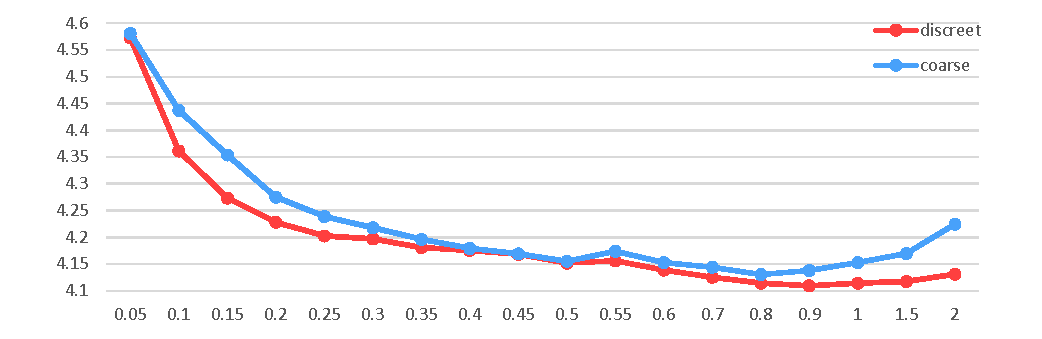
\includegraphics[width=0.5\linewidth]{eps2}
	}
	\subfloat[fixing $\varepsilon_{2}$ to values got above, varying $\varepsilon_{1}$ from 0 to 0.1]{
		\label{fig:epsilon:b}
		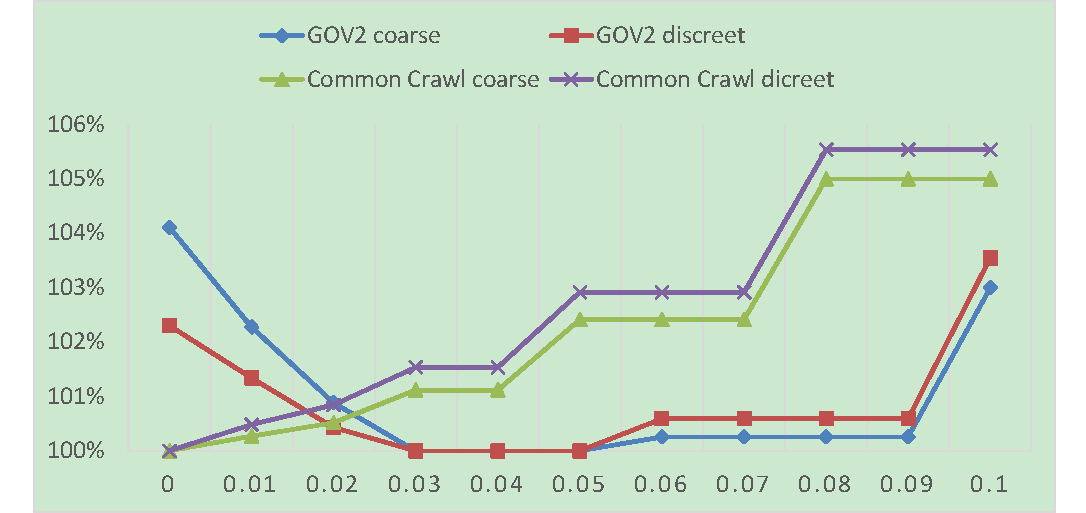
\includegraphics[width=0.5\linewidth]{eps1}
	}
	
	\caption{Influences of the parameters $\varepsilon_{2}$ and $\varepsilon_{1}$ on two partitioning strategies.}
	\label{fig:parameter}
\end{figure}

\begin{table}
	\caption{Configuration of parameters $ \left( \varepsilon_1, \varepsilon_2 \right) $ for different methods when compressing collections}
	\begin{center}
		\renewcommand{\arraystretch}{1.0}
		\setlength\tabcolsep{6pt}
		\begin{tabular}{*{3}c}
			\toprule
			& GOV2 & Common Crawl \\
			\midrule
			\textit{optimal} & $ \left(0.03, 0.3\right) $ & $ \left(0, 0.2\right) $\\
			\midrule
			\textit{coarse} & \multirow{2}*{$ \left(0.03, 0.8\right) $} & \multirow{2}*{$ \left(0, 0.7\right) $} \\
			\textit{discreet} & & \\
			\bottomrule
			\label{tab:parameter}
		\end{tabular}
	\end{center}
\end{table}

As mentioned in \cite{ottaviano2014partitioned}, only \textit{optimal} can benefit from parallelization.
Because finding an optimal partition is computationally intensive and requires much longer time, while the other methods, including \textit{coarse} and \textit{discreet}, are actually I/O-bound.
For the latter, thread switching might consume extra system resources.
In our experiment, parallelization prolongs construction times for these I/O-bound methods instead.
Even \textit{optimal} is accelerated, the procedure of finding the approximation parameters $ \left( \varepsilon_1, \varepsilon_2 \right) $ is still a repetitive work, which costs too much time.
Since \textit{coarse} and \textit{discreet} costs much less time, and works well on a single thread, this procedure is no longer a bottleneck.

\begin{table}
	\centering
	\caption{Comparison of construction time, and average bits per element of each component}
	\renewcommand{\arraystretch}{1.0}
	\setlength\tabcolsep{6pt}
	\begin{tabular}{@{}ll*{5}{r}}
		\toprule
		\multirow{2}*{collection} & \multirow{2}*{method} & \multicolumn{1}{c}{compress} &\multicolumn{1}{c}{size} & \multicolumn{1}{c}{docid} & \multicolumn{1}{c}{freq} & \multicolumn{1}{c}{decompress} \\
		& &\multicolumn{1}{c}{\textbf{sec}} & \multicolumn{1}{c}{\textbf{GB}} & \multicolumn{1}{c}{\textbf{bpi}} & \multicolumn{1}{c}{\textbf{bpi}} & \multicolumn{1}{c}{\textbf{sec}} \\
		\midrule
		\multirow{5}*{GOV2}
		& \textit{discreet} & 870.70 & 3.66 & 4.40 & 2.32 & 99.46 \\
		& \textit{coarse} & 785.94 & 3.73 & 4.55 & 2.34 & 99.09 \\
		& \textit{optimal} & 2638.91 & \textbf{3.38} & \textbf{4.05} & \textbf{2.19} & 86.11 \\
		\cmidrule(l){2-7}
		& \textit{uniform} & \textbf{251.63} & 3.80 & 4.63 & 2.40 & 80.54 \\
		& OptPFOR & 688.90 & 3.82 & 4.66 &2.41 & \textbf{49.43} \\
		\midrule
		\multirow{5}*{Common Crawl}
		& \textit{discreet} & 1926.84 & 11.30 & 7.54 & 3.03 & 178.64 \\
		& \textit{coarse} & 1873.80 & 11.34 & 7.63 & 3.04 & 180.20 \\
		& \textit{optimal} & 11983.70 & \textbf{10.81} & \textbf{7.35} & \textbf{2.83} & 177.89 \\
		\cmidrule(l){2-7}
		& \textit{uniform} & \textbf{645.95} & 11.44 & 7.73 & 3.05 & 187.42 \\
		& OptPFOR & 1520.90 & 11.64 & 7.86 &3.13 & \textbf{113.69} \\
		\bottomrule
		\label{tab:size and speed}
	\end{tabular}
\end{table}
% a vertical version, deprecated due to page width 
%\begin{table}
%	\caption{Comparison of construction time, and average bits per element of each component}
%	\begin{center}
%		\renewcommand{\arraystretch}{1.4}
%		\setlength\tabcolsep{6pt}
%		\begin{tabular}{c*{2}{*{2}{>{\columncolor[gray]{.9}}r}rr}}
%			\toprule
%			\multirow{3}*{methods}& \multicolumn{4}{c}{GOV2} & \multicolumn{4}{c}{Common Crawl} \\
%			\cmidrule(lr){2-5} \cmidrule(lr){6-9}
%			& \multicolumn{1}{c}{compress} & \multicolumn{1}{c}{docid} & \multicolumn{1}{c}{freq} & \multicolumn{1}{c}{decompress} & \multicolumn{1}{c}{compress} & \multicolumn{1}{c}{docid} & \multicolumn{1}{c}{freq} & \multicolumn{1}{c}{decompress} \\ 
%			& \multicolumn{1}{c}{\textbf{sec}} & \multicolumn{1}{c}{\textbf{bpi}} & \multicolumn{1}{c}{\textbf{bpi}} & \multicolumn{1}{c}{\textbf{sec}} & \multicolumn{1}{c}{\textbf{sec}} & \multicolumn{1}{c}{\textbf{bpi}} & \multicolumn{1}{c}{\textbf{bpi}} & \multicolumn{1}{c}{\textbf{sec}} \\
%			\midrule
%			\bottomrule
%			\label{tab:compression speed}
%		\end{tabular}
%	\end{center}
%\end{table}
\textit{Compression.} Table~\ref{tab:size and speed} shows the performances of different partitioning strategies on GOV2 and Common Crawl, adding OptPFOR-compressed index (OptPFOR) as a baseline.
Firstly we compare the construction time of these methods.
There is no doubt that \textit{uniform} gets the fastest speed on two collections, since it chooses the simplest partitioning strategy without extra calculations, even compared with OptPFOR, it still more than doubles the compression speed.
It is clear that both proposed strategies outperform the original ones by a large margin over the compression time, making construction of PEF competitive with OptPFOR, at the cost of a slight larger space occupancy.
Also note that compression time of most methods grows linearly as the collection size except \textit{optimal}.
From Table~\ref{tab:collection statistics}, we know that Common Crawl has nearly twice as many pointers as GOV2, however, \textit{optimal} costs 5 times longer time to compress.
This implies \textit{optimal} might not be a good choice for large collections in practice.

Next we compare the space occupancy using these methods.
Generally there is an inverse relationship between compressed size and compression time, however, the differences between each other are not statistically significant.
While inferior to \textit{optimal}, the two proposed methods are competitive compared with OptPFOR on both collections.
\textit{Discreet} has obvious superiority compared with \textit{coarse}, sacrificing 4.7\% construction time in exchange for 6\% smaller index size, however, it still gets a better compression ratio than the last two uniformly partitioned indexes.
The last column denotes time used for a sequential decompression of the index.
All EF-based indexes cost longer time than OptPFOR, and on GOV2 \textit{discreet} and \textit{coarse} tends to use 10\% longer time to traverse the index than \textit{optimal} and \textit{uniform}, when the collection gets larger, the differences tends to disappear.
Although all EF-based methods decompress much slower than OptPFOR, we will show in the following that their advantages are embodied in random access when applied to query processing.

\textit{Average partition length.} Table~\ref{tab:chunk size} shows comparisons of average partition lengths for different methods except \textit{uniform} and OptPFOR as they use fixed-sized block (128).
Results on GOV2 and Common Crawl are contrary to each other, we can notice that average partition length on GOV2 for \textit{optimal} is larger than \textit{coarse} and \textit{discreet}, nonetheless, smaller on Common Crawl.
It is likely caused by the local statistics of collections, for Common Crawl has fewer documents but more terms, \textit{docids} of its posting list trend to be more tightened together.
However, \textit{optimal} seems to find a more appropriate partition length.
Be it larger or smaller, will either lead to a decline of compression ratio.
\textit{Discreet} and \textit{coarse} do not differ much from each other, as they can only approximately locate an exception and build a chunk in front of it.
Next we show these lengths also influence query processing speed.
\begin{table}
	\centering
	\caption{Average partition lengths of different indexes for each component}
	\renewcommand{\arraystretch}{1.0}
	\begin{tabular}{@{}l*{4}{@{\extracolsep{1.5em}}r}}
		\toprule
		\multirow{2}*{} & \multicolumn{2}{c}{GOV2} & \multicolumn{2}{c}{Common Crawl} \\
		\cmidrule(lr){2-3} \cmidrule(lr){4-5}
		& \multicolumn{1}{c}{docid} & \multicolumn{1}{c}{freq} & \multicolumn{1}{c}{docid} & \multicolumn{1}{c}{freq} \\
		\midrule
		\textit{optimal} & 208 & 496 & 266 & 523 \\
		\textit{discreet} & 194 & 331 & 869 & 750 \\
		\textit{coarse} &187 & 319 & 651 & 784 \\
		\bottomrule
		\label{tab:chunk size}
	\end{tabular}
\end{table}

\subsection{Query efficiency}

In order to explore the efficiency differences caused by partitioning strategies, the experiment adopts four widely-used methods of ranked query to find the top-20 results, DAAT\_AND, DAAT\_OR, WAND and Maxscore.
% the differences of boolean query and dynamic pruning
Among these query processing strategies, the first two are exhaustive index traversal techniques without skipping, and the rest are two classic dynamic pruning techniques which allow skipping invalid blocks to reach an early termination.
Thus, we are able to compare the sequential decoding speed of these indexes using the first category and the support of random access using the second category.

% how we really build query set
%We randomly select 4000 terms from lexicon of the index, any of which has a document frequency within the range $(10^{5}, 10^{6})$, and we regroup them into 1000 queries every 4 terms, avoiding the bias brought by short posting lists while highlighting advantage of random access.
The query set if composed by 10000 queries of term number ranging from 1 to 5, with each kind accounting for 20\%.
All the queries are randomly sampled from TREC 2005 Efficiency Track topics, drawing only those whose terms have a mapping in the lexicon after stemming.
Also, the posting lists related to these queries have an average length larger than $ 10^5 $, avoiding the bias brought by short posting lists while highlighting advantage of random access.

% measuring in microseconds
Before performing queries, the whole inverted index is completely loaded into main memory, in order to avoid the confusion caused by disk I/O.
As declared in the beginning of this section, the query times, in milliseconds, are reported as the average of 4 consecutive replications.
% our goal is only to prove our methods are not obviously inferior to the original one.
Also note that our goal of this subsection is only to demonstrate that indexes built using our partitioning strategies are not obviously inferior to \textit{optimal}, since they are working in a much faster but less accurate way.
\begin{table}
	\centering
	\caption{Comparison of average query time in milliseconds under 4 query processing strategies}
	\renewcommand{\arraystretch}{1.0}
	\setlength\tabcolsep{6pt}
	\begin{tabular}{@{}ll*{4}{r}}
		\toprule
		\multirow{2}*{collection} & \multirow{2}*{method} & \multicolumn{4}{c}{query strategy} \\
		\cmidrule(lr){3-6}
		& &\multicolumn{1}{c}{DAAT\_AND} & \multicolumn{1}{c}{DAAT\_OR} & \multicolumn{1}{c}{WAND} & \multicolumn{1}{c}{Maxscore} \\
		\midrule
		\multirow{5}*{GOV2} 
		& \textit{discreet} & 4.05 & 34.41 & 6.64 & 13.89 \\
		& \textit{coarse}   & 4.12 & 34.53 & 6.68 & 14.01 \\
		& \textit{optimal}  & 3.87 & 33.49 & 6.22 & 13.20 \\
		\cmidrule(l){2-6}
		& \textit{uniform}  & 4.35 & 34.82 & 6.43 & \textbf{12.62} \\
		& OptPFOR  & \textbf{3.32} & \textbf{25.35} & \textbf{5.38} & 14.38 \\	
		\midrule
		\multirow{5}*{Common Crawl} 
		& \textit{discreet} & 4.06 & 35.18 & 14.25 & 25.32 \\
		& \textit{coarse}   & 4.10 & 35.64 & 14.29 & 25.33 \\
		& \textit{optimal}  & 4.06 & 34.78 & 14.19 & 25.16 \\
		\cmidrule(l){2-6}
		& \textit{uniform}  & 4.36 & 36.78 & 15.02 & \textbf{24.16} \\
		& OptPFOR  & \textbf{3.95} & \textbf{26.92} & \textbf{12.98} & 26.37 \\
		%		& discreet & 7.02 & 58.06 & 10.91 & 21.47 \\
		%		& coarse   & 8.10 & 56.32 & 11.33 & 22.61 \\
		%		\cmidrule(l){2-6}
		%		& optimal  & 6.52 & 55.27 & 13.25 & 21.14 \\
		%		& uniform  & 6.73 & 62.62 & 11.96 & 25.29 \\
		%		& OptPFOR  & 4.86 & 38.11 & 8.40 & 24.01 \\
		
		%		\multirow{5}*{GOV2} & discreet & 4099.48 & 35640.2 & 14251.4 & 25316.6 \\
		%		                      & coarse & 4061.74 & 35175.4 & 14287.3 & 25328.9 \\
		%		\cmidrule(l){2-6}
		%		  & optimal & 4056.39 & 34779.4 & 14189.8 & 25160.4 \\
		%		            & uniform & 4359.81 & 36780.1 & 15018.3 & 24156.8 \\
		%		            & OptPFOR & 3950.77 & 26916.7 & 12977.7 & 16369.9 \\
		%		\midrule
		%		\multirow{5}*{Common Crawl} & discreet & 7024.89 & 64324.7 & 10914.9 & 22614.9 \\
		%		                              & coarse & 8100.53 & 58062.9 & 11325.4 & 21466.7 \\
		%		\cmidrule(l){2-6}
		%		          & optimal & 6516.33 & 55272 & 13253.7 & 21137.7 \\
		%		                     & uniform & 6732.35 & 62617.6 & 11963.5 & 25288.1 \\
		%		                    & OptPFOR & 4863.62 & 38107.8 & 8396.07 & 12008.5 \\
		\bottomrule
		\label{tab:efficiency}
	\end{tabular}
\end{table}

First, we report the average query time of these indexes in Table~\ref{tab:efficiency}.
Again, performances of our methods are generally intermediate between that of \textit{optimal} and \textit{uniform}, and \textit{discreet} is always better than \textit{coarse}.
Among all the times reported by the four query strategies, our methods are slightly slower than \textit{optimal}, confirming the fact that the chosen partitions meet the requirement of fast decoding.
% AND and OR 在两个数据集中差不多,但在后面两个中差距变大
For the exhaustive traversal techniques, DAAT\_AND and DAAT\_OR, times are almost the same for both collections.
Since they need to scan the whole lists, their speeds are highly constrained by the length of the lists, and OptPFOR outperforms other methods due to its simple structure.
When it comes to dynamic pruning methods, results begin to diverge.
Times reported on GOV2 are half of those on Common Crawl for all the encoders, it is likely caused by the skipping of useless blocks, given the fact that Common Crawl contains more pointers and larger partition lengths, its performance on dynamic pruning methods is unsurprisingly less efficient.

% 最快的都是fixed-sized encoders
The best time achieved by these encoders are emphasized in bold, we can find traditional OptPFOR outperforms others in the first three cases, the edges ranges from 13\% to 24\%.
Even though it drops behind the three optimal partitioning strategies for Maxscore, another partitioning strategy with fixed-sized blocks, \textit{uniform}, becomes the best encoder.
Generally, optimal partitioning strategies focus on minimizing the compress sized rather than the query efficiency, its advantage of random access is based on building blocks aligning to dense cluster of docid and becomes obvious only when there are many long posting lists need to intersect.
%consistent with the observations made in PEF
The results here merely show our methods are competitive with the original one while sightly slower than partitioning strategies using fixed-sized blocks.
This observation is also consistent with that made in \cite{ottaviano2014partitioned}.

% 与表格基本一致,两个数据集表现差别不大
Next we use boxplot to display the distribution of query times, from which more details can be found beyond an average can offer.
As shown in Figure~\ref{fig:queries}, the boxplots for GOV2 and Common Crawl are actually very similar, except that times of dynamic pruning strategies on GOV2 are smaller than that on Common Crawl.
Overall, the figure is consistent with the average showed in Table~\ref{tab:efficiency}.

From the distribution, we can see most queries can be processed within 20 milliseconds, and query times of outliers are delayed by involvements of multiple long posting lists, which are at most 100 times larger than the minimum time.
Performances vary a lot among different processing methods, DAAT traverses the index exhaustively, its processing speed heavily relies only on the throughput of postings.
In detail, DAAT\_AND is the most efficient one as list intersection can cut off large of invalid postings, DAAT\_OR comes at a much higher cost as it cut nothing off, its rank also coincides with decompression speed shown in Table~\ref{tab:size and speed}.
When it comes to dynamic pruning, PEF begins to gain an advantage over OptPFOR, also performance gaps among indexes again become unapparent, \textit{discreet} and \textit{coarse} even outperform \textit{optimal} in WAND comparing both outliers and median.
In general, results of different indexes do not differ much except those using DAAT\_OR, performances of \textit{discreet} and \textit{coarse} rank between \textit{optimal} and \textit{uniform}.

An interesting phenomenon is that OptPFOR is more stable than other encoders, its query time distribution is compact for all the four query strategies.
Thus, the outliers represented as points make less difference to the average speed.
We can see for DAAT\_AND, the median almost stays the same, however, OptPFOR ranks the first of the average time due to its smaller outliers.
The reason can be twofold, first, fixed-sized block ensures a stable decoding time for all the posting lists; second, the underlying binary packing is more efficient to implement compared with \textit{uniform}.
Among the three optimal partitioning strategies, they do not differ from each other much when it comes to the distribution of query time.
\begin{figure}
	\centering
	\subfloat[GOV2]{
		\label{fig:query_gov2}
		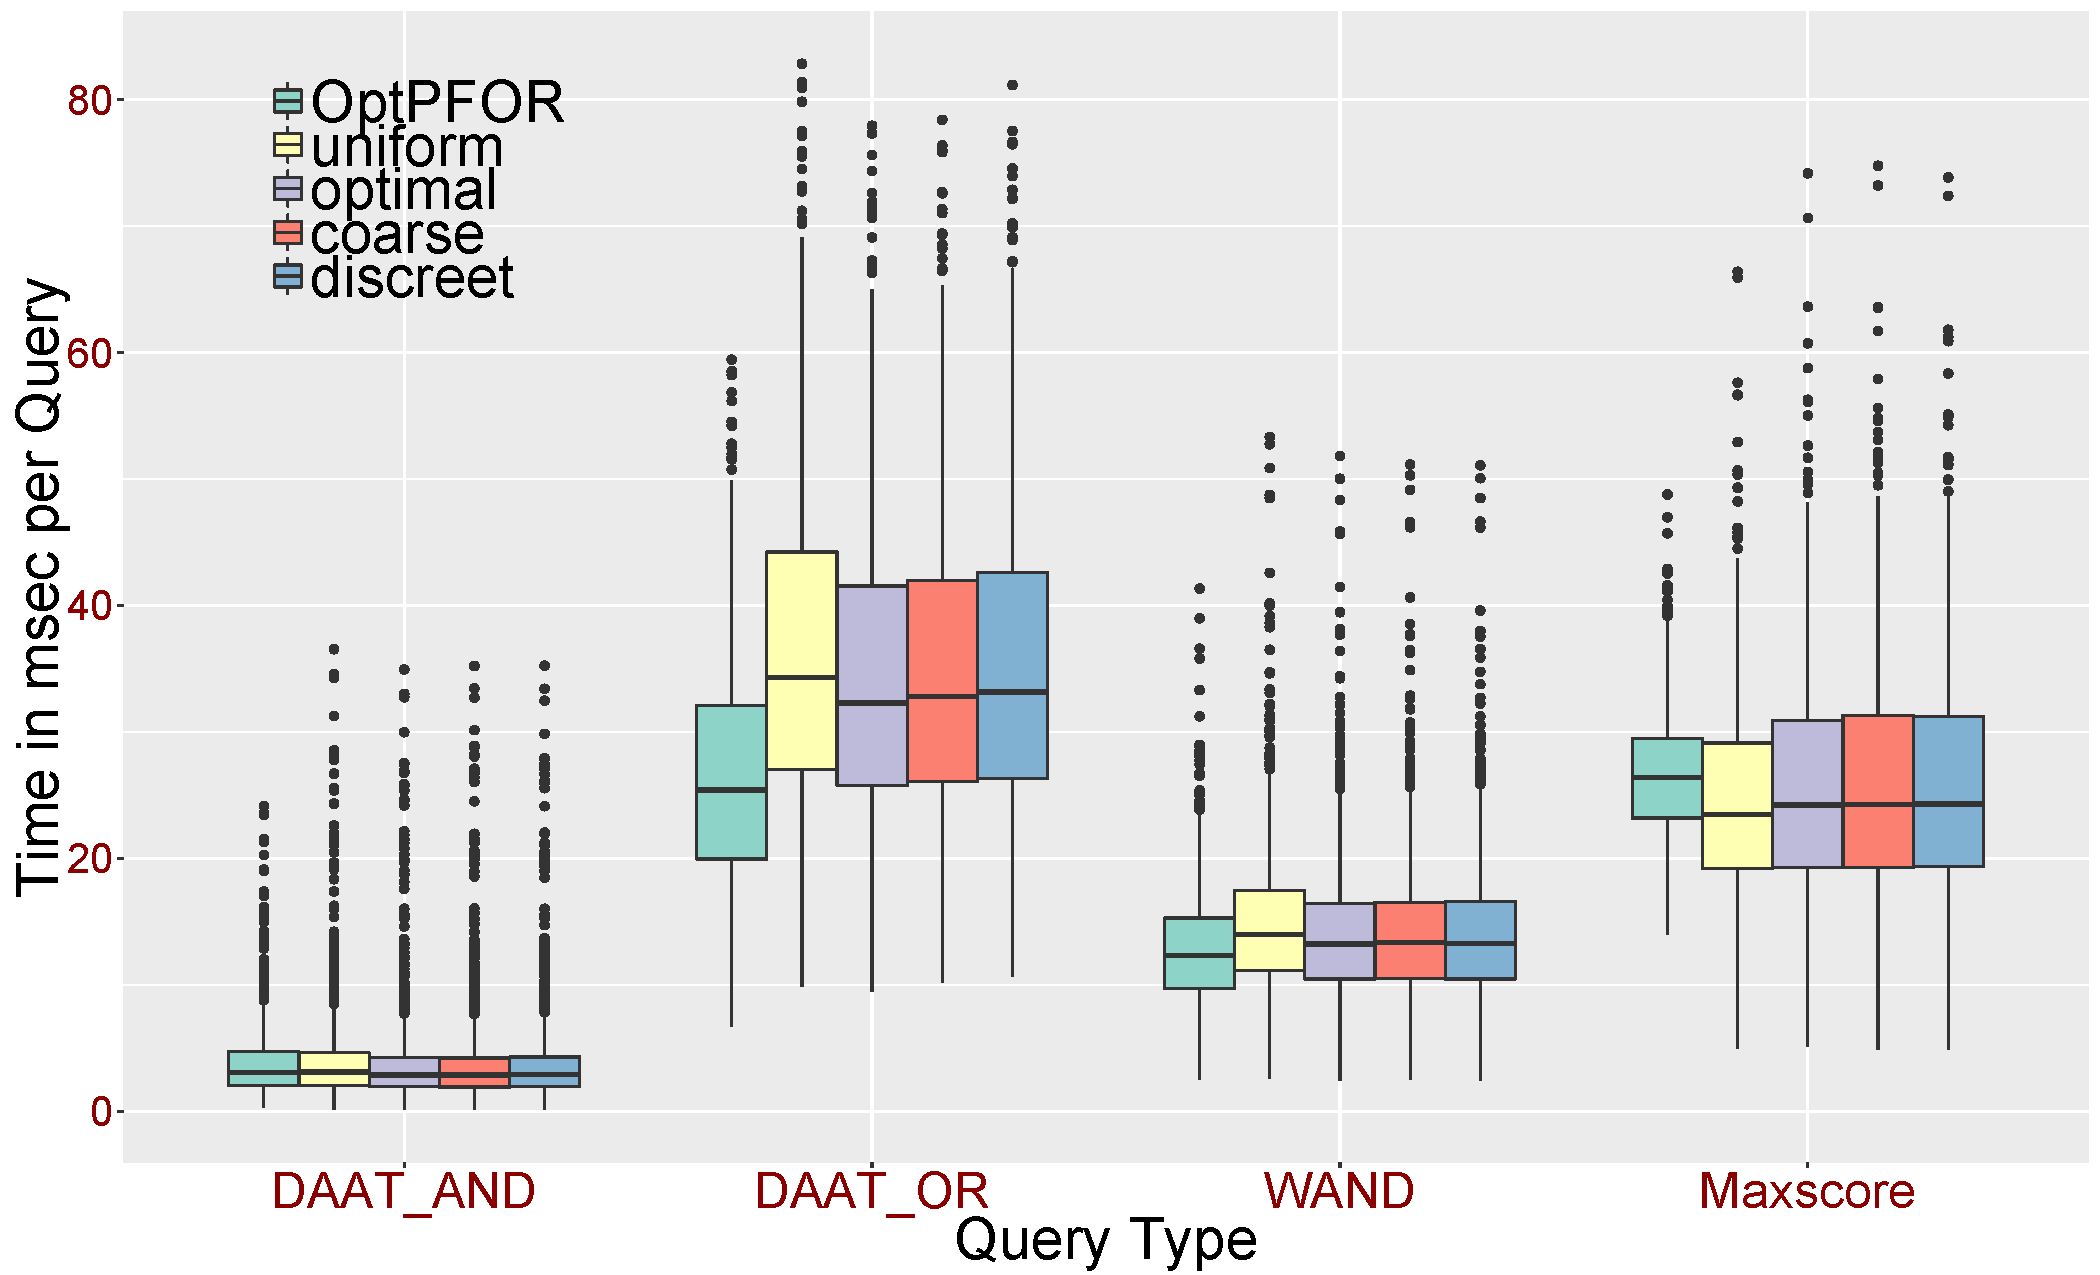
\includegraphics[width=0.5\linewidth]{queries_gov2}
	}
	\subfloat[Common Crawl]{
		\label{fig:query_cc}
		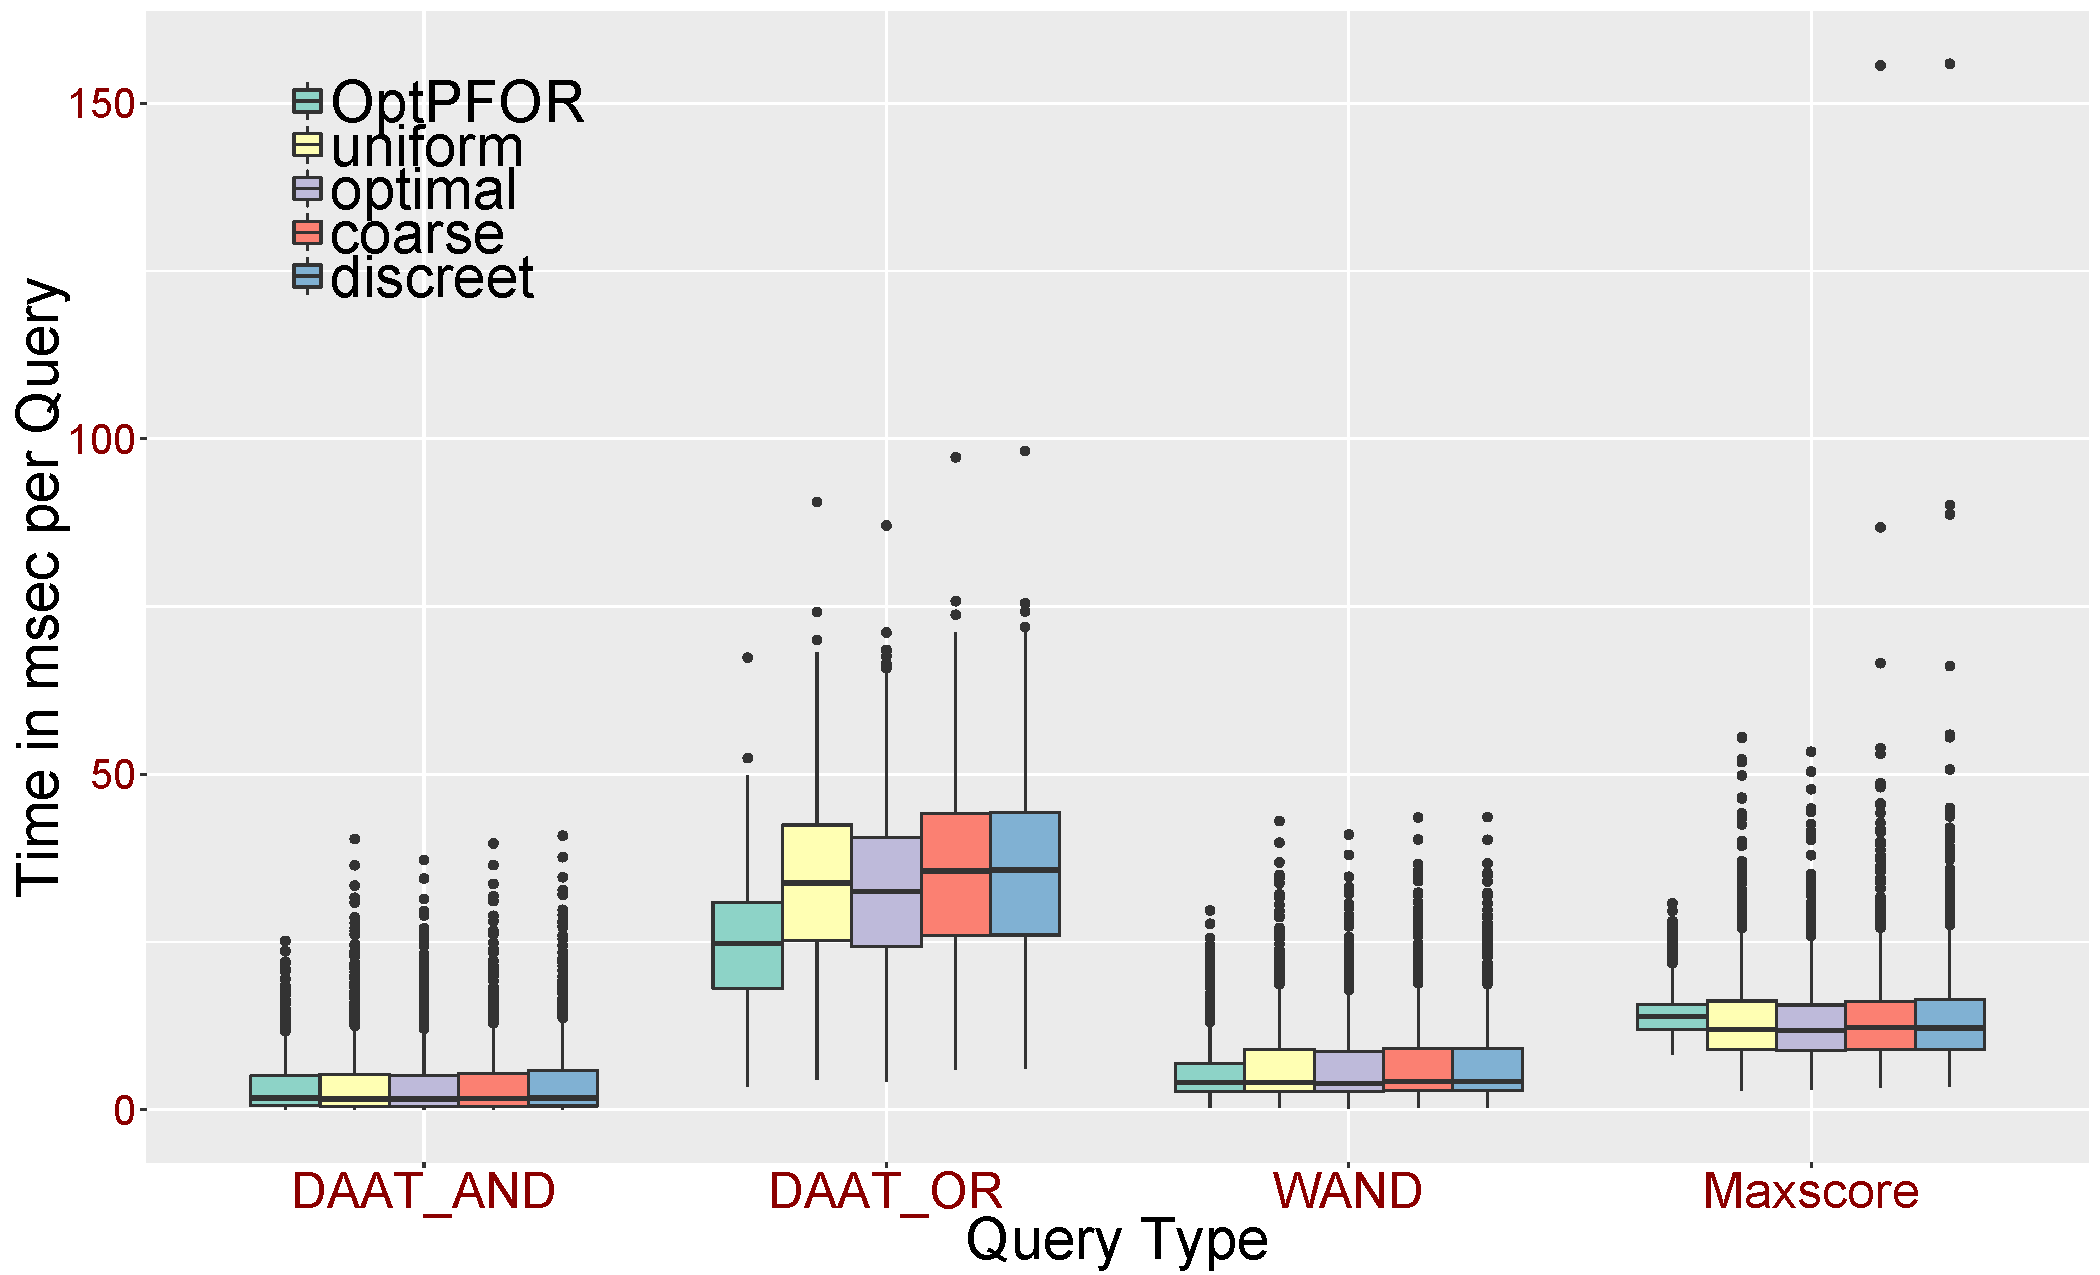
\includegraphics[width=0.5\linewidth]{queries_cc}
	}
	
	\caption{Query time distribution for different query processing methods on GOV2 and Common Crawl.}
	\label{fig:queries}
\end{figure}

\section{Conclusions and Future Work}\label{sec:conclusion}

In this paper, we have introduced the notion of Pareto-optimal compression techniques taking compression time as one criterion and compared performances of different compression techniques.
Based on the observation that Partitioned Elias-Fano index may cost too much time tuning the compression parameters, we proposed an optimization which heuristically partitions the posting lists to obtain an efficient compression while preserving the same approximation guarantees in space.
Experiments showed that our optimization sharply reduces the compression time of the original method, even makes it possible to be competitive with traditional OptPFOR.
Also, the compressed ratio is intermediate between \textit{optimal} and OptPFOR.

Even though the query efficiency get impaired accordingly, the latency is within an acceptable limit.
Generally, our work provides a trade-off between fast indexing and optimal compression, it suits the scenario where fast and effective compression is in demand and a slightly worse query efficiency is tolerable.
Since the partitioning strategy only focuses on optimal compression, what has been overlooked is the decoding speed of the built partition, future work will introduce a bicriteria combining both space cost and time weight to design a better partitioning strategy.

\bibliographystyle{splncs03}
\bibliography{reference}

\section*{Appendix: Deduction of reasonable partition length ratios}\label{sec:appendix}

%\appendix[Deduction of reasonable partition length ratios] 
Denote the two consecutive partitions starting from the same position as $ \mathcal{P}_{1}[ v_0, v_1 ] $ and $ \mathcal{P}_{2}[v_0, v_2] $.
Accordingly, their partition length and universe are $ n_1, u_1 $ and $ n_2, u_2 $, suppose $n_2 = n_1 + k, u_2 = u_1 + k + j $.
For completeness of exposition we report here the deduction of reasonable ratios for all the 9 combinations between $ \mathcal{E}[1] $ and $ \mathcal{E}[2] $, $ \mathcal{E} \in (0, 1, 2) $, showing that they asymptotically reach the same upper bound as their partition cost.
Shown as the following equation:

\begin{equation}
\sup\{\frac{n_2}{n_{1}}\} = {c\left(v_{0}, v_{2}\right)}/{c\left(v_{0}, v_{1}\right)}=\frac{c_2}{c_1}=1+\varepsilon_{2}
\end{equation}

\begin{enumerate}
	
	\item \label{itm:rb2rb}
	Both chunks are represented using \textit{bitvector}, $ \mathcal{E}[1] = \mathcal{E}[2] = 1 $.
	Then
	\begin{align*}
	c_2 & = u_2 & c_1 & = u_1 \\ 
	n_2 & > \frac{u_2}{4} &	n_1 & > \frac{u_1}{4}
	\end{align*}
	Since $ \frac{c_2}{c_1}=1+\varepsilon_2, n_2 = n_1 + k, u_2 = u_1 + k + j $, we get
	\begin{gather*}
	\frac{u_2}{u_1} = \frac{u_1+k+j}{u_1}=1+\varepsilon_2\\
	\frac{u_1+k+j}{n_1+k} < 4\\
	\frac{u_1}{n_1} < 4
	\end{gather*}
	Finally
	\begin{gather*}
	k+j<4k<4n_1\cdot \varepsilon_2 \\
	\frac{n_2}{n_1}=\frac{n_1+k}{n_1} < \frac{n_1+ n_1\cdot \varepsilon_2}{n_1}=1+\varepsilon_2
	\end{gather*}
	
	\item \label{itm:ef2ef}
	Both chunks are represented using EF, $ \mathcal{E}[1] = \mathcal{E}[2] = 2 $.
	Then
	\begin{align*}
	c_2 & = n_2(2+\lfloor \log \frac{u_2}{n_2} \rfloor) & c_1 & = n_1(2+\lfloor \log \frac{u_1}{n_1} \rfloor) \\ 
	n_2 & \leq \frac{u_2}{4} &	n_1 & \leq \frac{u_1}{4}
	\end{align*}
	Since
	\begin{gather*}
	\frac{n_2}{n_1} \cdot \frac{2+\lfloor \log \frac{u_2}{n_2} \rfloor}{2+\lfloor \log \frac{u_1}{n_1} \rfloor} = 1 + \varepsilon_2 \\ 
	\lfloor \log \frac{u_2}{n_2} \rfloor \geq 2 \Rightarrow \frac{2+\lfloor \log \frac{u_2}{n_2} \rfloor}{2+\lfloor \log \frac{u_1}{n_1} \rfloor} \approx 1
	\end{gather*}
	We get 
	\[
	\frac{n_2}{n_1} \approx 1+ \varepsilon_2 
	\]
	
	\item \label{itm:rb2ef}
	The former chunk is represented by \textit{bitvector} and the latter is EF, $ \mathcal{E}[1]= 1, \mathcal{E}[2]=2 $.
	Then
	\begin{align*}
	c_2 & = n_2(2+\lfloor \log \frac{u_2}{n_2} \rfloor) & c_1 & = u_1 \\ 
	n_2 & \leq \frac{u_2}{4} &	n_1 & > \frac{u_1}{4}
	\end{align*}
	Since
	\begin{gather*}
	\frac{n_2 \cdot (2+\lfloor \log \frac{u_2}{n_2} \rfloor)}{4 n_1} < \frac{n_2 \cdot (2+\lfloor \log \frac{u_2}{n_2} \rfloor)}{u_1} = 1 + \varepsilon_2 \\
	\frac{n_2}{n_1} \cdot \frac{2+\lfloor \log \frac{u_2}{n_2} \rfloor}{4} < 1 + \varepsilon_2
	\end{gather*}
	we get
	\[
	\frac{n_2}{n_1} \leq \frac{n_2}{n_1} \cdot \frac{2+\lfloor \log \frac{u_2}{n_2} \rfloor}{4} < 1 + \varepsilon_2
	\]
	
	\item \label{itm:ef2rb}
	The former chunk is represented by EF and the latter is \textit{bitvector}, $ \mathcal{E}[1]= 2, \mathcal{E}[2]=1 $.
	Then
	\begin{align*}
	c_2 & = u_2 & c_1 & = n_1(2+\lfloor \log \frac{u_1}{n_1} \rfloor)\\ 
	n_2 & > \frac{u_2}{4} & n_1 & \leq \frac{u_1}{4}
	\end{align*}
	Since
	\begin{gather*}
	\frac{4 n_2}{n_1 \cdot (2+\lfloor \log \frac{u_1}{n_2} \rfloor)} > \frac{n_2 \cdot (2+\lfloor \log \frac{u_2}{n_2} \rfloor)}{u_1} = 1 + \varepsilon_2 \\
	\frac{n_2}{n_1} \cdot \frac{4}{2+\lfloor \log \frac{u_1}{n_1} \rfloor} > 1 + \varepsilon_2
	\end{gather*}
	we get
	\[
	\frac{n_2}{n_1} \geq \frac{n_2}{n_1} \cdot \frac{2+\lfloor \log \frac{u_2}{n_2} \rfloor}{4} > 1 + \varepsilon_2
	\]
\end{enumerate}

Note that chunks represented using \textit{bitvector} are dense chunks, those using EF are sparser.
So in previous case~\ref{itm:rb2ef}, chunks change from dense to sparse, exceptions are certainly encountered in the middle.
As for case~\ref{itm:ef2rb}, chunks are becoming dense, it only happens under the situation without exceptions.

We do not analyze chunks represented using \textit{non-encoding}, as they extreme cases that are rarely encountered, and their partition weights are set to be zero which makes them more sensitive to exceptions.
Intuitively, \textit{non-encoding} cannot be leaded by EF or \textit{bitvector}, and it can be followed by the other two representations no matter how long its partition length is.
In extreme case, we can set every single integer to be represented by \textit{non-encoding}, however, it does not compress at all but produces many more chunks.
So we set the chunks which use \textit{non-encoding} to be at least longer than 8 integers and following the same upper bound as other cases.

Thus we set the partition length ratio to be $ 1+\varepsilon_2 $, and once $ \frac{n_2}{n_1} < 1+ \varepsilon_2 $ for two consecutive chunks starting from the same position, we can certainly determine that an exception is encountered in the middle.

%%%%%%%%%%%%%%%%%%%%%%%%%%%%%%%%%%%%%%%%%
%% For the final version of the paper: %%
%%%%%%%%%%%%%%%%%%%%%%%%%%%%%%%%%%%%%%%%%

%% Author information
%\vspace{4ex}\noindent
%\textbf{Author One} is\dots
%
%\bigskip\noindent
%\textbf{Author Two} is\dots
%
%\bigskip\noindent
%\textbf{Author Three} is\dots

%% Reception and acceptance information
%\bigskip
%\paragraph{Received: Month DD, 20YY; Accepted: Month DD, 20YY.}

\end{document}
